\begin{frame}{Arbre généalogique (encore) \gloss{Family tree (cont.)}}
  \begin{columns}[t]
    \column{0.5\textwidth}
      La famille de Jacques
      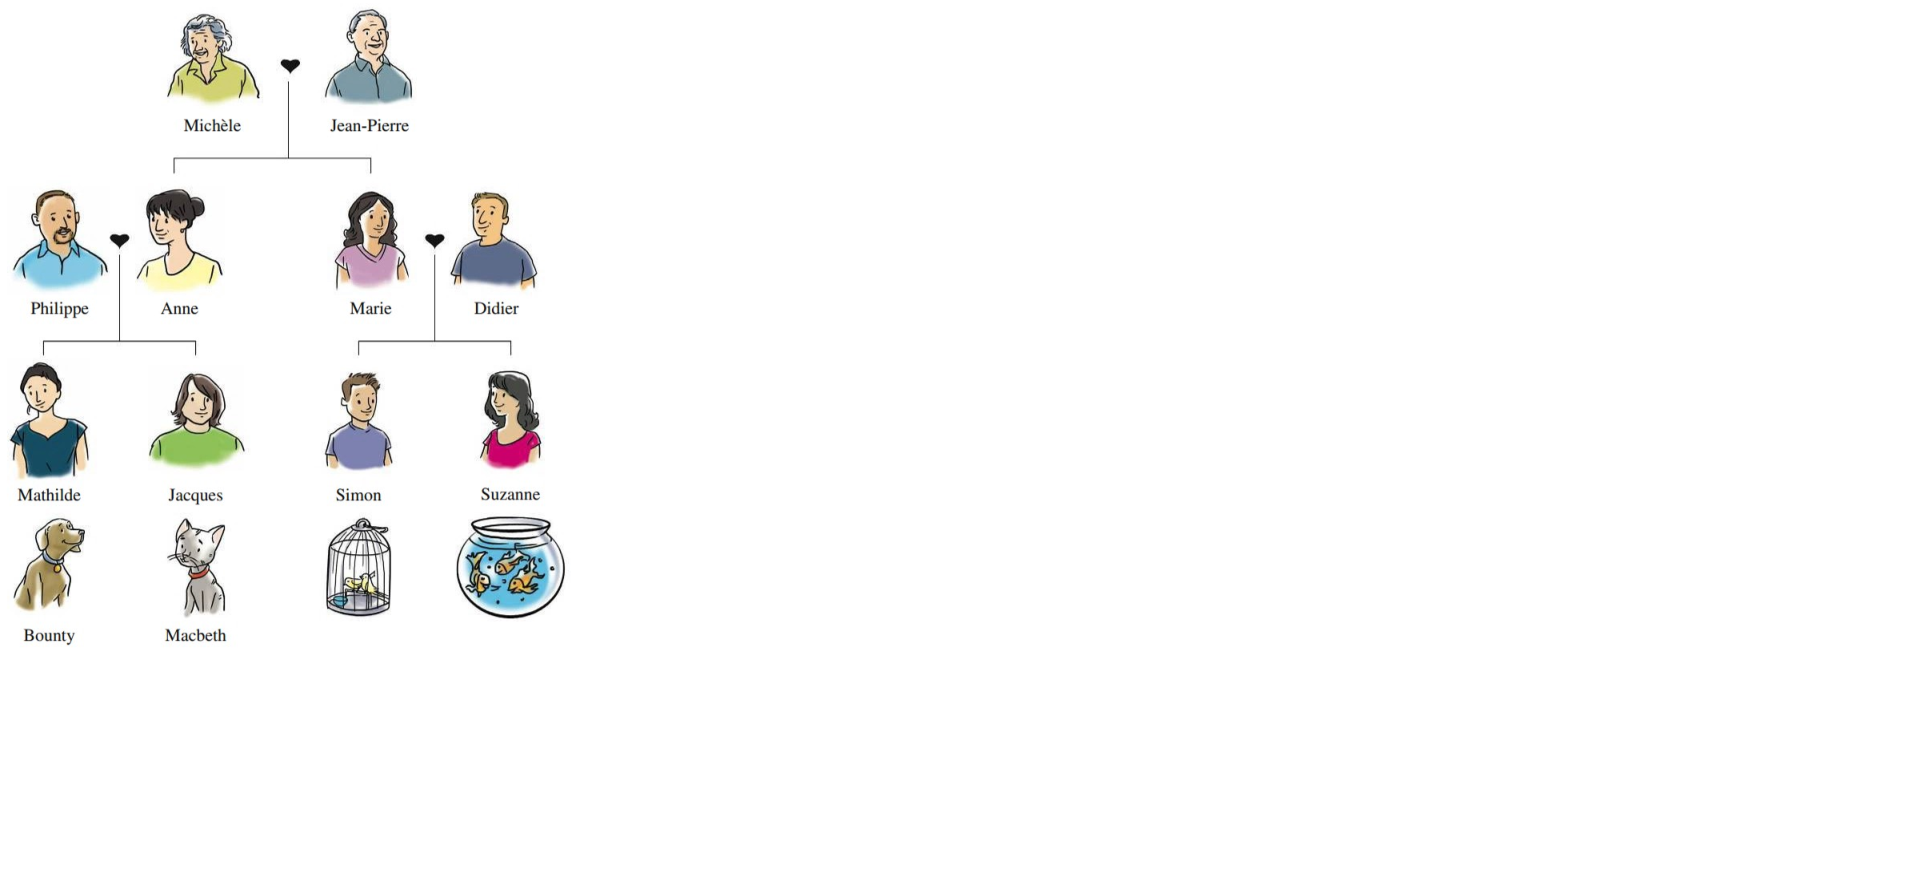
\includegraphics[scale=0.4]{famille_de_jacques.png}
    \column{0.5\textwidth}
      \small
      \gloss{In groups of 3 or 4, each person choose a family member in the tree to be, and take turns asking each other if they have a particular family member and, if so, that family member's name.
      For example:}
      \begin{itemize}
        \item[E1:] Est-ce que tu as une sœur?
        \item[] \tinygloss{Do you have a sister?}
        \item[E2:] Oui, j'ai une sœur.
        \item[] \tinygloss{Yes, I have a sister.}
        \item[E1:] Comment s'appelle ta sœur?
        \item[] \tinygloss{What is your sister's name?}
        \item[E2:] Ma sœur s'appelle ...
        \item[] \tinygloss{My sister's name is ...}
      \end{itemize}
  \end{columns}
\end{frame}